\chapter{D3.js – Data-Driven Documents}
\label{cha:d3js}

Chapter \ref{cha:d3js} provides an overview of the popular JavaScript library D3 which is used to simplify implementations of any data visualizations in the web for developers. The chapter provides an overview of the libraries beginnings but also goes into detail about how to implement projects with D3. The knowledge is required to understand the performance comparisons in chapter \ref{chap:performance} and \ref{chap:conclusion}.

\begin{figure}
    \centering
    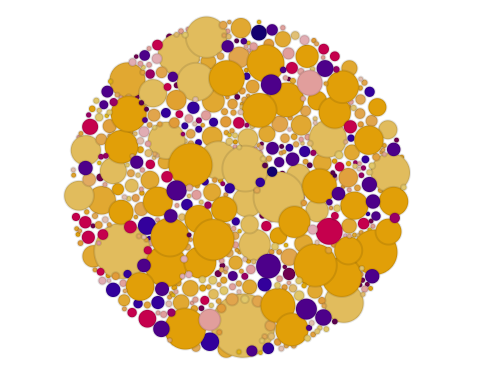
\includegraphics[width=0.5\columnwidth]{force001.PNG}
    \caption{The force graph with default center force. All nodes are attracted to the same center without overlapping each other.}
    \label{fig:force001}
  \end{figure}

\section{Introduction to D3}

D3 is a JavaScript library that helps developers create highly sophisticated data visualizations on the web via a universal tool that is platform agnostic: the browser. The official documentation of D3 in \cite[Introduction]{D3Website} explains the library as a toolkit, that allows binding data to the DOM. Also, it gives an overview of the vast amount of helpful tools that can be used to visualize data. The library includes all kinds of functionality, ranging from picking color ranges, choosing animation springs, randomizing numbers to rendering simple bar charts or calculating treemaps or real-time rendered force simulations.

\begin{figure}
  \centering
  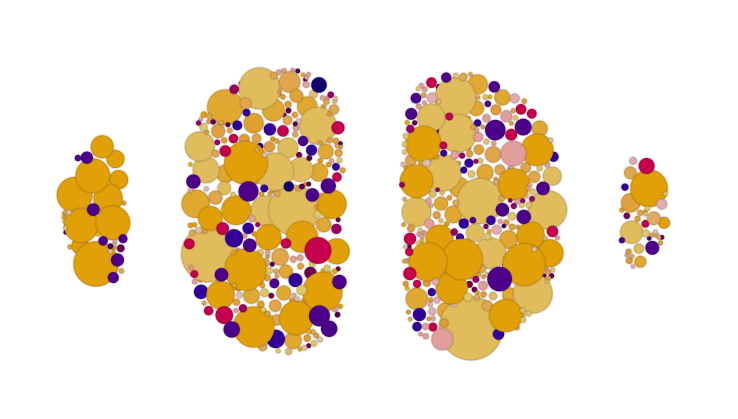
\includegraphics[width=0.6\columnwidth]{force002.PNG}
  \caption{A sample force graph with more than one center force. Having more than one force centers means that different nodes are attracted to their assigned center force.}
  \label{fig:force002}
\end{figure}

\begin{emergency}{1em}
There are multiple examples on the documentation's example page in \cite{D3Examples} which show what developers can achieve by using the D3 library. The API documentation is a comprehensive documentation of the complete feature set of D3 as seen in \cite[\mbox{/d3/blob/master/API.md}]{D3Github}. Due to the immense size of D3, the focus of this thesis and its project lies on a rather ''small'' but quite important part of the library -- the force graph simulation functionality.
\end{emergency}

\section{Force Graphs -- Real time rendered data visualizations}

This paper focuses on a special graph type which is called ''force simulation''. It is the graph type that is integrated into React as showcased by the thesis project. The visualizations consist of objects that interact with each other in a two-dimensional space. By interacting and moving objects all other objects in the animation are also affected. Figures \ref{fig:force001} and \ref{fig:force002} show an example of D3's force simulation. In figure \ref{fig:force001} there is a single center force that keeps all nodes in the center but also keeps individual nodes from overlapping each other. Force graphs can also be configured to make nodes reject each other even further than their actual size as figure \ref{fig:force004} shows. It is also possible to implement so-called links, that also add some complexity to the simulation, as nodes are dependent on each other and not only reject each other but also attract linked nodes as figure \ref{fig:force002} and \ref{fig:force005} shows.

\begin{figure}
    \centering
    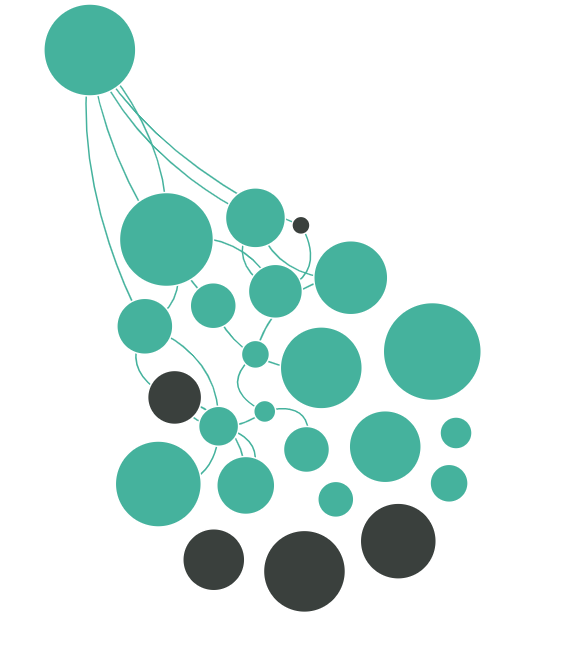
\includegraphics[width=0.4\columnwidth]{forceOwn002.PNG}
    \caption{A sample force graph where the top node is dragged up to the left and the other nodes are dragged along. The force is still keeping the other nodes apart and also drawn to the center though.}
    \label{fig:force003}
  \end{figure}

As previously mentioned, all force simulations are calculated, animated, and rendered in the browser which also includes user interaction. The user can for example drag nodes around which of course then affects other nodes and the whole simulation. Figure \ref{fig:force003} shows well, how dragging one node affects the whole force graph, as all connected nodes follow the dragged node while still rejecting each other and while being attracted to the center force.

D3 provides a somewhat simplified API to be able to quickly implement force graphs in the browser as it can be read in \cite[/d3-force/blob/master/README.md]{D3Github}. The way force simulations work is that developers first have to define or build the simulation. There is a factory method as seen in \hyperref[prog:simulation]{line 1} which takes the nodes of the graph as an argument and builds a default simulation. The nodes have to be provided in a particular scheme so D3 can correctly parse the node array. 

\begin{figure}
  \centering
  
\includegraphics[width=0.45\columnwidth]{forceOwn003.PNG}
  \caption{A sample force graph with one center force. The nodes are configured to reject each other with the function \texttt{r+r/2}}
  \label{fig:force004}
\end{figure}

\begin{program}
\caption{Code snippets for D3 force simulation code}
\label{prog:simulation}
\begin{JsCode}
simulation.forceSimulation([nodes]) // factory method for a standard force simulation
simulation.tick([iterations]) // called on every tick the simulation goes through
simulation.start() // starts a stopped simulation
simulation.stop() // stops a started simulation
simulation.restart() // restarts a simuliation, resets alpha
simulation.alpha([alpha]) // directly sets alpha value
simulation.alphaTarget([alphaTarget]) // sets alpha target value
\end{JsCode}
\end{program}

Another very important aspect of force graphs is the so called ''alpha'' value system as documented in \cite[/d3-force/blob/master/README.md]{D3Github}, which controls how long the simulation lives. The alpha valueis a gradually decaying value that makes the simulation stop if a certain value is reached. Every simulationhas a function that is called every ''tick'' of the simulation as shown in \hyperref[prog:simulation]{line 2}. Everytick the alpha value decays via a predefinable function, it happens logarithmically per default. The tickingfunction takes a handling function will be passed every node position in the simulation which then letsdevelopers link the data to the dom with D3 again. The tick function will be very important lateron when thecombination of D3 and React is explained in more detail.

\begin{figure}
    \centering
    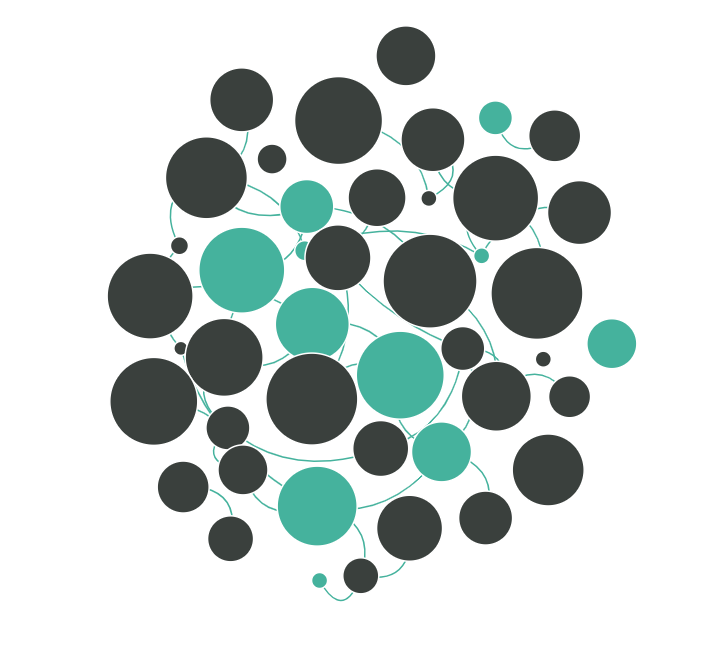
\includegraphics[width=0.45\columnwidth]{forceOwn001.PNG}
    \caption{A sample force graph where some nodes are linked together while still rejecting each other;}
    \label{fig:force005}
  \end{figure}

If there is a user interaction, the simulation sometimes has to be restarted or reheated. Programmers can set alpha values and targets to reheat or restart the simulation in case a node is dragged by the user which would possibly require many other nodes in the simulation to react to that user input. That way also the speed of the simulation can be controlled via setting a custom decay function. The documentation in \cite[/d3-force/blob/master/README.md]{D3Github} points to a few methods that can achieve said functionality. There is for example the functions which can be found in \hyperref[prog:simulation]{line 3}, \hyperref[prog:simulation]{line 4}, and \hyperref[prog:simulation]{line 5} that can be used to reheat a simulation. Also the functions in \hyperref[prog:simulation]{line 6} and \hyperref[prog:simulation]{line 7} values can be set directly to alter the simulation's life span.

%% add code snippets of pure D3

\section{History of D3}

%%The library was created in late 2010 according to the documentation in \cite{D3}. 

\section{Explaining the D3 API} 

\begin{itemize}
    \item Talk about chaining and how this is old scool
    \item Explain problems from chaining
    \item Explain how chaining might produce very unreadable code when used extensively
\end{itemize}